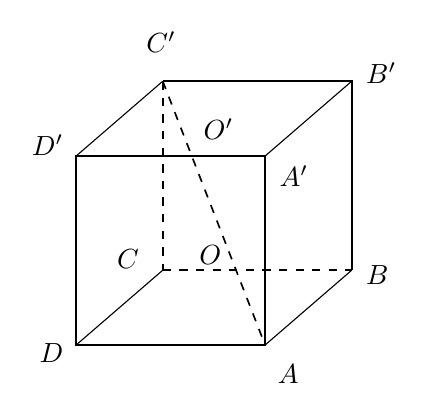
\begin{tikzpicture}[line width=.6pt,font=\normalsize,x=1cm,y=1cm]
\coordinate (D) at (0,0);
\coordinate (A) at (2.4,0);
\coordinate (Ap) at (2.4,2.4);
\coordinate (Dp) at (0,2.4);
\coordinate (C) at (1.1,0.95);
\coordinate (B) at (3.5,0.95);
\coordinate (Bp) at (3.5,3.35);
\coordinate (Cp) at (1.1,3.35);
\coordinate (O) at (1.958,1.139);
\coordinate (Op) at (1.36,2.68);
% front face
\draw (D) -- (A) -- (Ap) -- (Dp) -- cycle;
% back frame
\draw (Cp) -- (Bp) -- (B);
% receding edges (thin)
\draw[line width=.4pt] (Dp) -- (Cp);
\draw[line width=.4pt] (Ap) -- (Bp);
\draw[line width=.4pt] (D) -- (C);
\draw[line width=.4pt] (A) -- (B);
% hidden edges
\draw[dashed] (Cp) -- (C);
\draw[dashed] (C) -- (B);
% body diagonal C'A
\draw[dashed] (Cp) -- (A);
\node[anchor=east, inner sep=1.5pt] at (-0.1,2.54) {$D'$};
\node[anchor=south, inner sep=1.5pt] at (1.08,3.65) {$C'$};
\node[anchor=west, inner sep=1.5pt] at (3.62,3.45) {$B'$};
\node[anchor=west, inner sep=1.5pt] at (2.52,2.14) {$A'$};
\node[anchor=east, inner sep=1.5pt] at (0.86,1.098) {$C$};
\node[anchor=west, inner sep=1.5pt] at (3.62,0.89) {$B$};
\node[anchor=east, inner sep=1.5pt] at (-0.1,-0.1) {$D$};
\node[anchor=north west, inner sep=1.5pt] at (2.5,-0.18) {$A$};
\node[anchor=west, inner sep=1.5pt] at (1.557,2.737) {$O'$};
\node[left=2pt, inner sep=1pt] at (O) {$O$};
\end{tikzpicture}
